\documentclass[8pt,aspectratio=169]{beamer}
\usetheme{Madrid}
\usepackage{graphicx}
\usepackage{booktabs}
\usepackage{adjustbox}
\usepackage{multicol}
\usepackage{amsmath}
\usepackage{amssymb}
\usepackage{tikz}
\usetikzlibrary{arrows.meta,positioning,shapes.callouts,shapes.geometric,decorations.pathreplacing}
\usepackage{colortbl}
\usepackage{pgfplots}
\pgfplotsset{compat=1.18}
\usepackage{hyperref}
\usepackage{algorithm}
\usepackage{algorithmic}

% Color definitions
\definecolor{mlblue}{RGB}{0,102,204}
\definecolor{mlpurple}{RGB}{51,51,178}
\definecolor{mllavender}{RGB}{173,173,224}
\definecolor{mllavender2}{RGB}{193,193,232}
\definecolor{mllavender3}{RGB}{204,204,235}
\definecolor{mllavender4}{RGB}{214,214,239}
\definecolor{mlorange}{RGB}{255, 127, 14}
\definecolor{mlgreen}{RGB}{44, 160, 44}
\definecolor{mlred}{RGB}{214, 39, 40}
\definecolor{mlgray}{RGB}{127, 127, 127}

% Additional colors for template compatibility
\definecolor{lightgray}{RGB}{240, 240, 240}
\definecolor{midgray}{RGB}{180, 180, 180}
\definecolor{dfteal}{RGB}{0,128,128}
\definecolor{dfred}{RGB}{180,30,30}

% Backward compatibility: uppercase color names
\colorlet{MLPurple}{mlpurple}
\colorlet{MLBlue}{mlblue}
\colorlet{MLOrange}{mlorange}
\colorlet{MLGreen}{mlgreen}
\colorlet{MLRed}{mlred}
\colorlet{MLLavender}{mllavender}
\colorlet{MLGray}{mlgray}

% Apply custom colors to Madrid theme
\setbeamercolor{palette primary}{bg=mllavender3,fg=mlpurple}
\setbeamercolor{palette secondary}{bg=mllavender2,fg=mlpurple}
\setbeamercolor{palette tertiary}{bg=mllavender,fg=white}
\setbeamercolor{palette quaternary}{bg=mlpurple,fg=white}

\setbeamercolor{structure}{fg=mlpurple}
\setbeamercolor{section in toc}{fg=mlpurple}
\setbeamercolor{subsection in toc}{fg=mlblue}
\setbeamercolor{title}{fg=mlpurple}
\setbeamercolor{frametitle}{fg=mlpurple,bg=mllavender3}
\setbeamercolor{block title}{bg=mllavender2,fg=mlpurple}
\setbeamercolor{block body}{bg=mllavender4,fg=black}

% Remove navigation symbols
\setbeamertemplate{navigation symbols}{}

% Clean itemize/enumerate
\setbeamertemplate{itemize items}[circle]
\setbeamertemplate{enumerate items}[default]

% Reduce margins for more content space
\setbeamersize{text margin left=5mm,text margin right=5mm}

% Custom course footer
\setbeamertemplate{footline}{
  \leavevmode%
  \hbox{%
    \begin{beamercolorbox}[wd=.333333\paperwidth,ht=2.25ex,dp=1ex,center]{author in head/foot}%
      \usebeamerfont{author in head/foot}Methods and Algorithms
    \end{beamercolorbox}%
    \begin{beamercolorbox}[wd=.333333\paperwidth,ht=2.25ex,dp=1ex,center]{title in head/foot}%
      \usebeamerfont{title in head/foot}MSc Data Science
    \end{beamercolorbox}%
    \begin{beamercolorbox}[wd=.333333\paperwidth,ht=2.25ex,dp=1ex,right]{date in head/foot}%
      \usebeamerfont{date in head/foot}\insertframenumber{} / \inserttotalframenumber\hspace*{2ex}
    \end{beamercolorbox}}%
  \vskip0pt%
}

% Command for bottom annotation (Madrid-style)
\newcommand{\bottomnote}[1]{%
\vfill
\vspace{-2mm}
\textcolor{mllavender2}{\rule{\textwidth}{0.4pt}}
\vspace{1mm}
\footnotesize
\textbf{#1}
}

% Custom commands for course compatibility
\newcommand{\highlight}[1]{\textcolor{mlorange}{\textbf{#1}}}
\newcommand{\mathbold}[1]{\boldsymbol{#1}}

% Compact list environment
\newenvironment{compactlist}{%
  \begin{itemize}%
    \setlength{\itemsep}{2pt}%
    \setlength{\parskip}{0pt}%
    \setlength{\parsep}{0pt}%
}{%
  \end{itemize}%
}

\title[L06c: Embeddings \& LLMs]{From Words to Worlds: Embeddings in the Age of LLMs}
\subtitle{How Computers Went from Reading Words to Understanding Language}
\author{Prof.\ Dr.\ J\"org Osterrieder}
\institute{Methods and Algorithms --- MSc Data Science}
\date{Spring 2026}

\begin{document}

%% ===== FRONT MATTER (3 slides) =====

% Slide 1: Title Page
\begin{frame}[plain]
\titlepage
\end{frame}

% Slide 2: XKCD Opening
\begin{frame}{How Did We Get Here?}
\begin{columns}[c]
\begin{column}{0.45\textwidth}
\centering
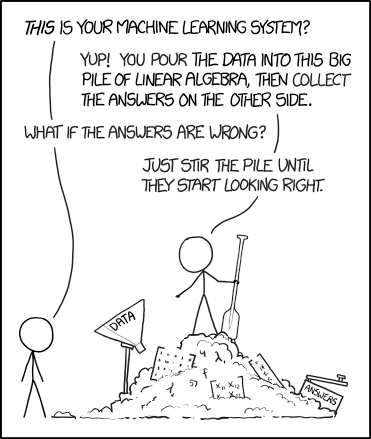
\includegraphics[height=0.55\textheight]{images/1838_machine_learning.png}
\end{column}
\begin{column}{0.50\textwidth}
\large
How did we go from computers that can't read\ldots\ to ChatGPT?

\vspace{6mm}
Today we trace the journey: from simple word vectors to large language models.
\end{column}
\end{columns}
\bottomnote{XKCD \#1838 by Randall Munroe (CC BY-NC 2.5).}
\end{frame}

% Slide 3: Learning Objectives
\begin{frame}{Learning Objectives}
\vspace{3mm}
By the end of this lecture you will be able to:
\vspace{4mm}
\begin{enumerate}
  \setlength{\itemsep}{6pt}
  \item \textbf{Explain} what word embeddings do and why they matter
  \item \textbf{Identify} the limit of static embeddings (polysemy)
  \item \textbf{Describe} how LLMs use contextual embeddings to understand language
\end{enumerate}
\bottomnote{Everything is explained with pictures and analogies.}
\end{frame}

%% ===== ACT 1: THE PROBLEM + STATIC EMBEDDINGS (5 slides) =====

% Slide 4: TikZ Comic C1 --- Lost in Translation 2.0
\begin{frame}{The Problem: Can Computers Really Understand Us?}
\centering
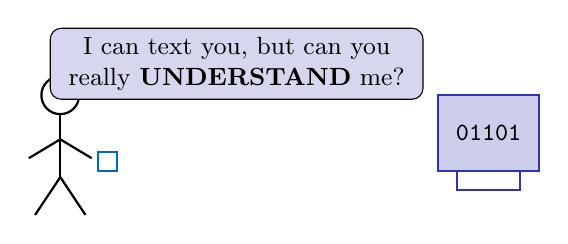
\begin{tikzpicture}[scale=0.8]
  % Stick figure
  \draw[thick] (-3,1.5) circle (0.3);
  \draw[thick] (-3,1.2) -- (-3,0.2);
  \draw[thick] (-3,0.8) -- (-3.5,0.5);
  \draw[thick] (-3,0.8) -- (-2.5,0.5);
  \draw[thick] (-3,0.2) -- (-3.4,-0.4);
  \draw[thick] (-3,0.2) -- (-2.6,-0.4);
  % Phone in hand
  \draw[thick,mlblue] (-2.4,0.6) rectangle (-2.1,0.3);
  % Speech bubble
  \node[draw,rounded corners,fill=mllavender4,text width=4.5cm,align=center,font=\small]
    at (-0.2,2.0) {I can text you, but can you really \textbf{UNDERSTAND} me?};
  % Computer
  \draw[thick,mlpurple,fill=mllavender3] (3.0,0.3) rectangle (4.6,1.5);
  \node[font=\ttfamily\small] at (3.8,0.9) {01101};
  \draw[thick,mlpurple] (3.3,0.0) rectangle (4.3,0.3);
\end{tikzpicture}

\vspace{3mm}
Computers see characters. We need them to understand \highlight{meaning}.
\bottomnote{From Siri to ChatGPT --- it all starts with turning words into numbers.}
\end{frame}

% Slide 5: CHART --- Word Embedding Space
\begin{frame}{Words as Points in Space}
\begin{columns}[c]
\begin{column}{0.60\textwidth}
\centering

\includegraphics[width=0.95\textwidth]{01_word_embedding_space/chart.pdf}
\end{column}
\begin{column}{0.38\textwidth}
\begin{compactlist}
  \item Word2Vec solved this --- words become \highlight{points in space}
  \item Similar words cluster together
  \item The computer learned these positions by reading text
\end{compactlist}
\end{column}
\end{columns}
\bottomnote{Word2Vec (2013) was the breakthrough: learn word meaning from context.}
\end{frame}

% Slide 6: CHART --- Word Analogy
\begin{frame}{The ``Aha Moment'': Vector Arithmetic on Words}
\begin{columns}[c]
\begin{column}{0.58\textwidth}
\centering

\includegraphics[width=0.95\textwidth]{top10_08_word_analogy/chart.pdf}
\end{column}
\begin{column}{0.40\textwidth}
\begin{compactlist}
  \item King $-$ Man $+$ Woman $=$ Queen
  \item Paris $-$ France $+$ Germany $=$ Berlin
  \item Embeddings capture relationships as \highlight{vector arithmetic}
\end{compactlist}
\end{column}
\end{columns}
\bottomnote{This is the ``aha moment'': meaning has direction in embedding space.}
\end{frame}

% Slide 7: CHART --- Similarity Heatmap
\begin{frame}{Measuring Word Similarity}
\begin{columns}[c]
\begin{column}{0.58\textwidth}
\centering

\includegraphics[width=0.95\textwidth]{02_similarity_heatmap/chart.pdf}
\end{column}
\begin{column}{0.40\textwidth}
\begin{compactlist}
  \item Dark squares = similar words
  \item Light squares = unrelated words
  \item The computer learned this from text alone
\end{compactlist}
\end{column}
\end{columns}
\bottomnote{Cosine similarity measures the angle between word vectors. Small angle = similar meaning.}
\end{frame}

% Slide 8: TikZ Comic C2 --- The Dictionary Analogy
\begin{frame}{Static Embeddings = A Dictionary}
\centering
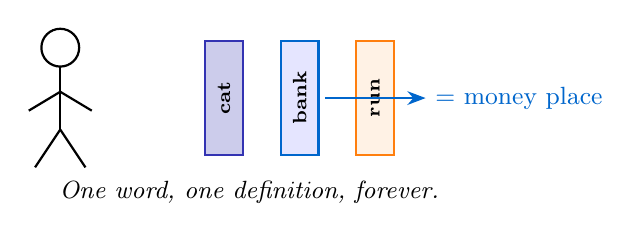
\begin{tikzpicture}[scale=0.8]
  % Stick figure
  \draw[thick] (-3.5,1.5) circle (0.3);
  \draw[thick] (-3.5,1.2) -- (-3.5,0.2);
  \draw[thick] (-3.5,0.8) -- (-4.0,0.5);
  \draw[thick] (-3.5,0.8) -- (-3.0,0.5);
  \draw[thick] (-3.5,0.2) -- (-3.9,-0.4);
  \draw[thick] (-3.5,0.2) -- (-3.1,-0.4);
  % Three books
  \draw[thick,mlpurple,fill=mllavender3] (-1.2,-0.2) rectangle (-0.6,1.6);
  \node[rotate=90,font=\scriptsize\bfseries] at (-0.9,0.7) {cat};
  \draw[thick,mlblue,fill=blue!10] (0.0,-0.2) rectangle (0.6,1.6);
  \node[rotate=90,font=\scriptsize\bfseries] at (0.3,0.7) {bank};
  \draw[thick,mlorange,fill=orange!10] (1.2,-0.2) rectangle (1.8,1.6);
  \node[rotate=90,font=\scriptsize\bfseries] at (1.5,0.7) {run};
  % Arrow from "bank" to definition
  \draw[-{Stealth},thick,mlblue] (0.7,0.7) -- (2.3,0.7);
  \node[right,font=\small,mlblue] at (2.3,0.7) {= money place};
  % Caption
  \node[font=\small\itshape] at (-0.5,-0.8) {One word, one definition, forever.};
\end{tikzpicture}

\vspace{3mm}
Word2Vec gives each word \highlight{ONE fixed vector}. Great for analogies.\\
But is one definition enough?
\bottomnote{Static embeddings: fast, efficient, but frozen. Every use of ``bank'' maps to the same point.}
\end{frame}

%% ===== ACT 2: GOING DEEPER + THE LIMIT (5 slides) =====

% Slide 9: CHART --- Word Frequency
\begin{frame}{How Models Learn: Word Frequency Patterns}
\begin{columns}[c]
\begin{column}{0.58\textwidth}
\centering

\includegraphics[width=0.95\textwidth]{top10_11_word_frequency_rank/chart.pdf}
\end{column}
\begin{column}{0.40\textwidth}
\begin{compactlist}
  \item Words follow Zipf's law (few common, many rare)
  \item Embeddings learn from word co-occurrence patterns
  \item LLMs read trillions of words --- they see every pattern
\end{compactlist}
\end{column}
\end{columns}
\bottomnote{The more text a model reads, the better its embeddings. LLMs read the entire internet.}
\end{frame}

% Slide 10: CHART --- Embedding Dimensions
\begin{frame}{More Dimensions = More Nuance}
\begin{columns}[c]
\begin{column}{0.58\textwidth}
\centering

\includegraphics[width=0.95\textwidth]{top10_10_embedding_dimensions/chart.pdf}
\end{column}
\begin{column}{0.40\textwidth}
\begin{compactlist}
  \item More dimensions = more nuance in meaning
  \item This chart shows up to 50 dimensions
  \item BERT uses 768 dimensions. GPT-4 uses over 12,000
\end{compactlist}
\end{column}
\end{columns}
\bottomnote{Dimension count is a key difference: Word2Vec uses 100--300, modern LLMs use thousands.}
\end{frame}

% Slide 11: CHART --- Context Window
\begin{frame}{The Context Window: How Far Can a Model See?}
\begin{columns}[c]
\begin{column}{0.58\textwidth}
\centering

\includegraphics[width=0.95\textwidth]{top10_12_context_window/chart.pdf}
\end{column}
\begin{column}{0.40\textwidth}
\begin{compactlist}
  \item Word2Vec looks at a small context window (5--10 words)
  \item Bigger windows = better embeddings
  \item What if you could look at \highlight{everything} at once?
\end{compactlist}
\end{column}
\end{columns}
\bottomnote{Word2Vec: 5--10 word window. BERT: 512 tokens. GPT-4: 128,000 tokens.}
\end{frame}

% Slide 12: CHART --- Embedding PCA
\begin{frame}{Embeddings Have Internal Structure}
\begin{columns}[c]
\begin{column}{0.58\textwidth}
\centering

\includegraphics[width=0.95\textwidth]{top10_18_embedding_pca_variance/chart.pdf}
\end{column}
\begin{column}{0.40\textwidth}
\begin{compactlist}
  \item Embeddings have internal structure
  \item A few principal components capture most meaning
  \item LLMs build richer, deeper structure with more layers
\end{compactlist}
\end{column}
\end{columns}
\bottomnote{PCA reveals that embeddings are not random --- they encode linguistic structure.}
\end{frame}

% Slide 13: The Big Problem --- Polysemy
\begin{frame}{But Wait --- One Word, Many Meanings!}
\vspace{2mm}
\begin{center}
\large
``I deposited money at the \highlight{bank}''\\[6mm]
``I sat on the river \highlight{bank}''
\end{center}

\vspace{4mm}
Word2Vec gives \textbf{both} sentences the exact same vector for ``bank''.\\
That's clearly wrong! The word means completely different things.

\vspace{4mm}
\begin{block}{The Polysemy Problem}
This is called \textbf{polysemy} --- and static embeddings can't handle it.
\end{block}

\bottomnote{Polysemy (many meanings) is everywhere: ``run'' has 645 definitions in the dictionary.}
\end{frame}

%% ===== ACT 3: CONTEXTUAL EMBEDDINGS -> LLMs (5 slides) =====

% Slide 14: Transition
\begin{frame}{What If Embeddings Could Change?}
\vspace{8mm}
\begin{center}
{\Large What if ``bank'' near ``river'' got a \highlight{DIFFERENT} vector\\[3mm]
than ``bank'' near ``money''?}

\vspace{8mm}
{\large What if the embedding could read the surrounding words and \textbf{adapt}?}

\vspace{8mm}
\highlight{This is exactly what contextual embeddings do.}
\end{center}
\bottomnote{The key insight of 2018: embeddings should depend on context, not just the word itself.}
\end{frame}

% Slide 15: TikZ Comic C3 --- The Conversation
\begin{frame}{Context Changes Everything}
\centering
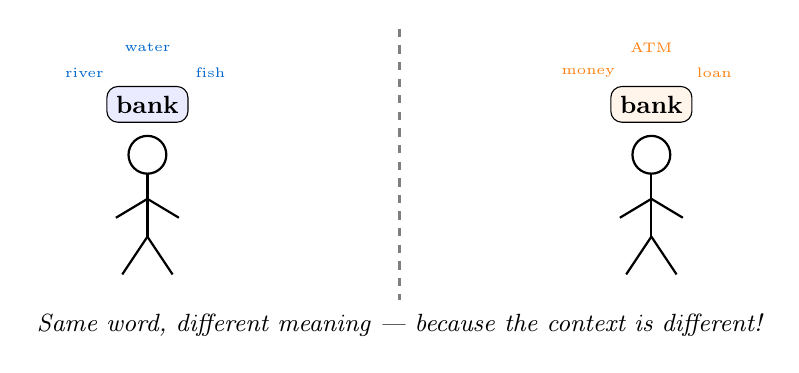
\begin{tikzpicture}[scale=0.8]
  % Left figure
  \draw[thick] (-4.0,1.5) circle (0.3);
  \draw[thick] (-4.0,1.2) -- (-4.0,0.2);
  \draw[thick] (-4.0,0.8) -- (-4.5,0.5);
  \draw[thick] (-4.0,0.8) -- (-3.5,0.5);
  \draw[thick] (-4.0,0.2) -- (-4.4,-0.4);
  \draw[thick] (-4.0,0.2) -- (-3.6,-0.4);
  % Left bubble
  \node[draw,rounded corners,fill=blue!8,font=\small\bfseries] at (-4.0,2.3) {bank};
  \node[font=\tiny,mlblue] at (-5.0,2.8) {river};
  \node[font=\tiny,mlblue] at (-3.0,2.8) {fish};
  \node[font=\tiny,mlblue] at (-4.0,3.2) {water};
  % Dashed separator
  \draw[dashed,thick,mlgray] (0,3.5) -- (0,-0.8);
  % Right figure
  \draw[thick] (4.0,1.5) circle (0.3);
  \draw[thick] (4.0,1.2) -- (4.0,0.2);
  \draw[thick] (4.0,0.8) -- (3.5,0.5);
  \draw[thick] (4.0,0.8) -- (4.5,0.5);
  \draw[thick] (4.0,0.2) -- (3.6,-0.4);
  \draw[thick] (4.0,0.2) -- (4.4,-0.4);
  % Right bubble
  \node[draw,rounded corners,fill=orange!8,font=\small\bfseries] at (4.0,2.3) {bank};
  \node[font=\tiny,mlorange] at (3.0,2.8) {money};
  \node[font=\tiny,mlorange] at (5.0,2.8) {loan};
  \node[font=\tiny,mlorange] at (4.0,3.2) {ATM};
  % Caption
  \node[font=\small\itshape] at (0,-1.2) {Same word, different meaning --- because the context is different!};
\end{tikzpicture}

\vspace{2mm}
Contextual embeddings compute a \highlight{new vector every time}, based on surrounding words.
\bottomnote{BERT (2018) and GPT (2018) were the first widely successful contextual embedding models.}
\end{frame}

% Slide 16: TikZ Diagram D1 --- Self-Attention
\begin{frame}{How It Works: Words Talk to Each Other}
\centering
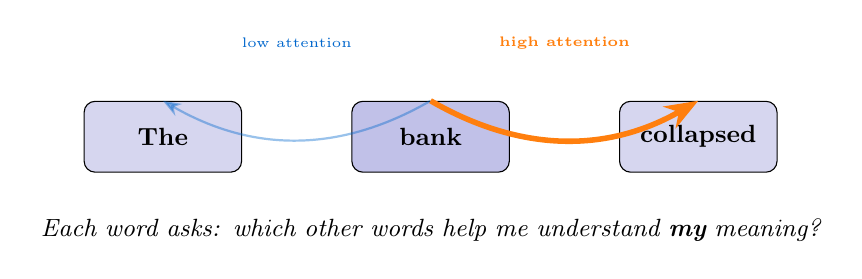
\begin{tikzpicture}[scale=0.85,
  box/.style={draw,rounded corners,minimum width=2cm,minimum height=0.9cm,
              fill=mllavender4,font=\small\bfseries}]
  \node[box] (the) at (-4,0) {The};
  \node[box,fill=mllavender2] (bank) at (0,0) {bank};
  \node[box] (col) at (4,0) {collapsed};
  % Attention arrows
  \draw[-{Stealth},thick,mlblue,opacity=0.4] (bank.north) to[bend left=30] (the.north);
  \draw[-{Stealth},line width=2pt,mlorange] (bank.north) to[bend right=30] (col.north);
  % Labels
  \node[font=\tiny,mlblue] at (-2.0,1.4) {low attention};
  \node[font=\tiny,mlorange] at (2.0,1.4) {\textbf{high attention}};
  % Caption
  \node[font=\small\itshape,text width=10cm,align=center] at (0,-1.4)
    {Each word asks: which other words help me understand \textbf{my} meaning?};
\end{tikzpicture}

\vspace{3mm}
This is called \textbf{self-attention}: every word looks at every other word to decide its meaning.
\bottomnote{Attention is the core mechanism of transformers --- the architecture behind BERT and GPT.}
\end{frame}

% Slide 17: TikZ Diagram D2 --- 3-Step Flowchart
\begin{frame}{How Contextual Embeddings Work}
\centering
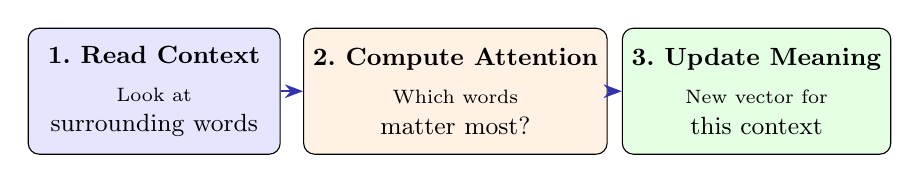
\begin{tikzpicture}[scale=0.85,
  sbox/.style={draw,rounded corners,minimum width=3.2cm,minimum height=1.6cm,
               fill=mllavender4,align=center,font=\small}]
  \node[sbox,fill=blue!10] (s1) at (-4.5,0)
    {\textbf{1.\ Read Context}\\[1mm]\scriptsize Look at\\surrounding words};
  \node[sbox,fill=orange!10] (s2) at (0,0)
    {\textbf{2.\ Compute Attention}\\[1mm]\scriptsize Which words\\matter most?};
  \node[sbox,fill=green!10] (s3) at (4.5,0)
    {\textbf{3.\ Update Meaning}\\[1mm]\scriptsize New vector for\\this context};
  \draw[-{Stealth},thick,mlpurple] (s1) -- (s2);
  \draw[-{Stealth},thick,mlpurple] (s2) -- (s3);
\end{tikzpicture}

\vspace{5mm}
That's it. Read context, weigh importance, update the embedding. Repeat for every word.
\bottomnote{BERT reads all words at once. GPT reads left-to-right. Both use attention to weigh which words matter most.}
\end{frame}

% Slide 18: Static vs Contextual Comparison Table
\begin{frame}{Static vs Contextual: What Changed?}
\vspace{2mm}
\centering
{\small
\begin{tabular}{l c c}
\toprule
\textbf{Aspect} & \textbf{Static (Word2Vec)} & \textbf{Contextual (BERT/GPT)} \\
\midrule
Vector     & One per word, fixed     & New one each time     \\
Model size & Small ($\sim$100\,MB)   & Large ($\sim$1--100\,GB) \\
Year       & 2013                    & 2018+                 \\
``bank''   & Always same vector      & Different per context \\
Example    & Word2Vec, GloVe         & BERT, GPT-4           \\
\bottomrule
\end{tabular}
}

\vspace{6mm}
\highlight{Same fundamental idea} (words as vectors), but now they're \textbf{dynamic}.
\bottomnote{The jump from static to contextual was the single biggest leap in NLP history.}
\end{frame}

%% ===== ACT 4: THE LLM REVOLUTION + APPLICATIONS (4 slides) =====

% Slide 19: TikZ Diagram D3 --- Scaling Timeline
\begin{frame}{The Scaling Story: Same Idea, Bigger Models}
\centering
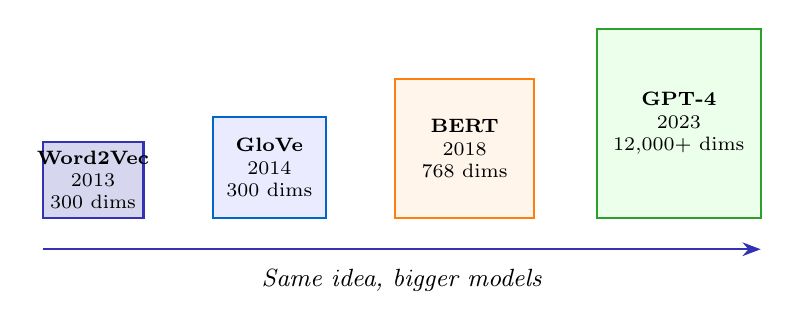
\begin{tikzpicture}[scale=0.8]
  % Boxes (progressively larger)
  \draw[thick,mlpurple,fill=mllavender4] (-5.2,0) rectangle (-3.6,1.2);
  \node[font=\scriptsize,align=center] at (-4.4,0.6) {\textbf{Word2Vec}\\2013\\300 dims};
  \draw[thick,mlblue,fill=blue!8] (-2.5,0) rectangle (-0.7,1.6);
  \node[font=\scriptsize,align=center] at (-1.6,0.8) {\textbf{GloVe}\\2014\\300 dims};
  \draw[thick,mlorange,fill=orange!8] (0.4,0) rectangle (2.6,2.2);
  \node[font=\scriptsize,align=center] at (1.5,1.1) {\textbf{BERT}\\2018\\768 dims};
  \draw[thick,mlgreen,fill=green!8] (3.6,0) rectangle (6.2,3.0);
  \node[font=\scriptsize,align=center] at (4.9,1.5) {\textbf{GPT-4}\\2023\\12,000+ dims};
  % Arrow underneath
  \draw[-{Stealth},thick,mlpurple] (-5.2,-0.5) -- (6.2,-0.5);
  \node[font=\small\itshape] at (0.5,-1.0) {Same idea, bigger models};
\end{tikzpicture}
\bottomnote{GPT-3 has 175 billion parameters. GPT-4 is estimated at over 1 trillion.}
\end{frame}

% Slide 20: What Can LLMs Do?
\begin{frame}{What Can LLMs Do?}
\vspace{2mm}
\begin{compactlist}
  \item \textcolor{mlpurple}{\textbf{Generate text}} --- write emails, reports, code
  \item \textcolor{mlblue}{\textbf{Answer questions}} --- from documents, databases, knowledge
  \item \textcolor{mlorange}{\textbf{Translate}} --- between languages, styles, formats
  \item \textcolor{mlgreen}{\textbf{Reason}} --- multi-step logic, math, planning
\end{compactlist}

\vspace{4mm}
\begin{block}{One Foundation}
All built on the same foundation: \textbf{embeddings + attention}.
\end{block}
\bottomnote{Every capability of ChatGPT traces back to contextual embeddings and self-attention.}
\end{frame}

% Slide 21: LLMs in Finance
\begin{frame}{LLMs in Finance}
\begin{columns}[t]
\begin{column}{0.47\textwidth}
\textcolor{mlpurple}{\textbf{Understanding}}
\begin{compactlist}
  \item Sentiment analysis of earnings calls
  \item ESG report classification
  \item Contract similarity search
\end{compactlist}
\end{column}
\begin{column}{0.47\textwidth}
\textcolor{mlblue}{\textbf{Acting}}
\begin{compactlist}
  \item Automated report generation
  \item Document Q\&A for compliance
  \item Market news summarization
\end{compactlist}
\end{column}
\end{columns}

\vspace{4mm}
\begin{block}{Key Insight}
Every LLM application starts with \textbf{embeddings}.
\end{block}
\bottomnote{Bloomberg, JPMorgan, and Goldman Sachs all deploy LLMs for financial text analysis.}
\end{frame}

% Slide 22: The Python Recipe
\begin{frame}[fragile]{Try It Yourself}
\begin{columns}[t]
\begin{column}{0.47\textwidth}
\textcolor{mlpurple}{\textbf{Classic (Word2Vec)}}
\vspace{2mm}

{\small
\texttt{from gensim.models import Word2Vec}\\[1pt]
\texttt{model = Word2Vec(sentences,}\\[1pt]
\texttt{~~~~~~~~~~~~~~~~vector\_size=100)}\\[1pt]
\texttt{model.wv.most\_similar("bank")}
}
\end{column}
\begin{column}{0.47\textwidth}
\textcolor{mlblue}{\textbf{Modern (OpenAI API)}}
\vspace{2mm}

{\small
\texttt{from openai import OpenAI}\\[1pt]
\texttt{client = OpenAI()}\\[1pt]
\texttt{response = client.embeddings.create(}\\[1pt]
\texttt{~~input="bank loan application",}\\[1pt]
\texttt{~~model="text-embedding-3-small")}
}
\end{column}
\end{columns}

\vspace{5mm}
\centering
2013: train your own.\quad 2024: call an API.
\bottomnote{Classic: pip install gensim. Modern: pip install openai (requires API key).}
\end{frame}

%% ===== CLOSING (3 slides) =====

% Slide 23: TikZ Comic C4 --- From Dictionary to Conversation Partner
\begin{frame}{The Journey: From Dictionary to Conversation Partner}
\centering
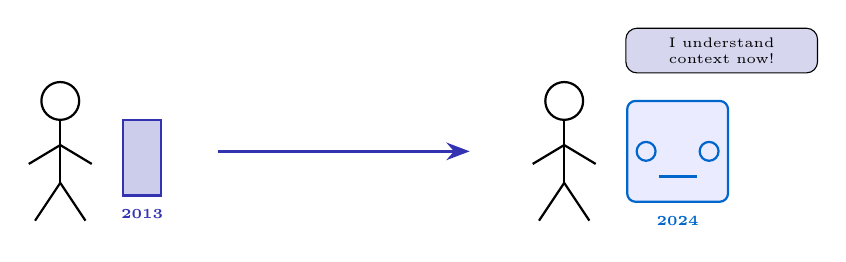
\begin{tikzpicture}[scale=0.8]
  % Left: stick figure + book (2013)
  \draw[thick] (-5.0,1.5) circle (0.3);
  \draw[thick] (-5.0,1.2) -- (-5.0,0.2);
  \draw[thick] (-5.0,0.8) -- (-5.5,0.5);
  \draw[thick] (-5.0,0.8) -- (-4.5,0.5);
  \draw[thick] (-5.0,0.2) -- (-5.4,-0.4);
  \draw[thick] (-5.0,0.2) -- (-4.6,-0.4);
  % Book
  \draw[thick,mlpurple,fill=mllavender3] (-4.0,0.0) rectangle (-3.4,1.2);
  \node[font=\tiny,mlpurple] at (-3.7,-0.3) {\textbf{2013}};
  % Arrow
  \draw[-{Stealth},very thick,mlpurple] (-2.5,0.7) -- (1.5,0.7);
  % Right: stick figure + robot (2024)
  \draw[thick] (3.0,1.5) circle (0.3);
  \draw[thick] (3.0,1.2) -- (3.0,0.2);
  \draw[thick] (3.0,0.8) -- (2.5,0.5);
  \draw[thick] (3.0,0.8) -- (3.5,0.5);
  \draw[thick] (3.0,0.2) -- (2.6,-0.4);
  \draw[thick] (3.0,0.2) -- (3.4,-0.4);
  % Robot
  \draw[thick,mlblue,fill=blue!8,rounded corners=3pt] (4.0,-0.1) rectangle (5.6,1.5);
  \draw[thick,mlblue] (4.3,0.7) circle (0.15);
  \draw[thick,mlblue] (5.3,0.7) circle (0.15);
  \draw[thick,mlblue] (4.5,0.3) -- (5.1,0.3);
  \node[draw,rounded corners,fill=mllavender4,font=\tiny,text width=2.2cm,align=center]
    at (5.5,2.3) {I understand context now!};
  \node[font=\tiny,mlblue] at (4.8,-0.4) {\textbf{2024}};
\end{tikzpicture}
\bottomnote{The same core idea --- words as vectors --- but now with context, scale, and understanding.}
\end{frame}

% Slide 24: Key Takeaways
\begin{frame}{Five Things to Remember}
\vspace{2mm}
\begin{enumerate}
  \setlength{\itemsep}{5pt}
  \item Embeddings turn words into \textbf{meaningful numbers}
  \item Static embeddings: one vector per word --- fast but miss context
  \item Contextual embeddings (BERT/GPT): new vectors based on surrounding words
  \item LLMs = contextual embeddings scaled to \textbf{billions of parameters}
  \item Every AI language tool --- from search to ChatGPT --- is built on embeddings
\end{enumerate}
\bottomnote{From 300 dimensions to 12,000+. From megabytes to terabytes. Same core idea.}
\end{frame}

% Slide 25: XKCD Closing
\begin{frame}{Go Teach a Machine Something}
\vspace{2mm}
\centering
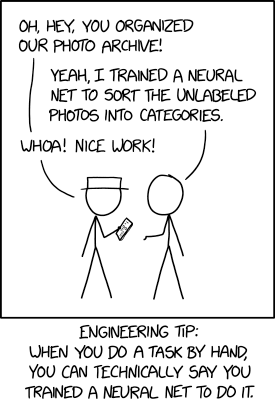
\includegraphics[height=0.55\textheight]{images/2173_trained_a_neural_net.png}
\bottomnote{XKCD \#2173 by Randall Munroe (CC BY-NC 2.5). Next: try the Jupyter notebook to build your own embeddings!}
\end{frame}

\end{document}
